%% abtex2-modelo-slides.tex, v-1.0 gfabinhomat
%% Copyright 2012-<COPYRIGHT_YEAR> by abnTeX2 group at http://www.abntex.net.br/ 
%%
%% This work may be distributed and/or modified under the
%% conditions of the LaTeX Project Public License, either version 1.3
%% of this license or (at your option) any later version.
%% The latest version of this license is in
%%   http://www.latex-project.org/lppl.txt
%% and version 1.3 or later is part of all distributions of LaTeX
%% version 2005/12/01 or later.
%%
%% This work has the LPPL maintenance status `maintained'.
%% 
%% The Current Maintainer of this work is Fábio Rodrigues Silva, 
%% member of abnTeX2 team, led by Lauro César Araujo. 
%% Further information are available on 
%% http://www.abntex.net.br/
%%
%% This work consists of the files abntex2-modelo-slides.tex, 
%% abntex2-modelo-references.bib and abntex2-modelo-marca.pdf
%%
%% Modelo desenvolvido por Fábio Rodrigues Silva (gfabinhomat@gmail.com)
%% Mais informações podem ser obtidas no guia do usuário Beamer 
%% (http://linorg.usp.br/CTAN/macros/latex/contrib/beamer/doc/beameruserguide.pdf)
%% Informações rápidas podem ser acessadas em http://en.wikibooks.org/wiki/LaTeX/Presentations


% Apresentações em widescreen. Outros valores possíveis: 1610, 149, 54, 43 e 32.
% Por padrão, as apresentações são no formato 4:3 (sem o aspectratio).
\documentclass[aspectratio=169]{beamer}	 	

\usetheme{Pittsburgh}
\usecolortheme{default}
\usefonttheme[onlymath]{serif}			% para fontes matemáticas
% Enconte mais temas e cores em http://www.hartwork.org/beamer-theme-matrix/ 
% Veja também http://deic.uab.es/~iblanes/beamer_gallery/index.html

% colors from github.com/paulgp/beamer-tips/blob/master/slides.tex
\definecolor{blue}{RGB}{0,114,178}
\definecolor{red}{RGB}{213,94,0}
\definecolor{yellow}{RGB}{240,228,66}
\definecolor{green}{RGB}{0,158,115}


% Customizações de Cores: fg significa cor do texto e bg é cor do fundo
\setbeamercolor{normal text}{fg=black}
\setbeamercolor{alerted text}{fg=red}
\setbeamercolor{author}{fg=blue}
\setbeamercolor{institute}{fg=blue}
\setbeamercolor{date}{fg=green}
\setbeamercolor{frametitle}{fg=red}
\setbeamercolor{framesubtitle}{fg=brown}
\setbeamercolor{block title}{bg=blue, fg=white}		%Cor do título
\setbeamercolor{block body}{bg=gray, fg=darkgray}	%Cor do texto (bg= fundo; fg=texto)

% ---
% PACOTES
% ---
\usepackage[alf]{abntex2cite}		% Citações padrão ABNT
\usepackage[brazil]{babel}		% Idioma do documento
\usepackage{color}			% Controle das cores
\usepackage[T1]{fontenc}		% Selecao de codigos de fonte.
\usepackage{graphicx}			% Inclusão de gráficos
\usepackage[utf8]{inputenc}		% Codificacao do documento (conversão automática dos acentos)
\usepackage{txfonts}			% Fontes virtuais
% ---
\usepackage{tikz}
\usetikzlibrary{positioning}
\usetikzlibrary{fit}

% --- Informações do documento ---
\title{Uso de aprendizado de máquina para beamforming aeroacústico}
\author{Guilherme Hiroshi Sinoara}
\institute{Universidade de São Paulo
	    \par
	    Escola de Engenharia de São Carlos}
\date{27 de janeiro de 2025}
% ---

\newcommand{\fautor}{Fonte: Elaborada pelo autor.}
\newcommand{\iu}{\mathrm{i}}

\setbeamercovered{transparent}

% ----------------- INÍCIO DO DOCUMENTO --------------------------------------
\begin{document}

% ----------------- NOVO SLIDE --------------------------------
\begin{frame}

\begin{minipage}{1\linewidth}
  \centering
  \begin{tabular}{cc}
    \begin{tabular}{c}
      \textbf{Universidade de São Paulo} \\
      \textbf{Escola de Engenharia de São Carlos}
    \end{tabular}
  \end{tabular}
\end{minipage}

\titlepage

\end{frame}

% ----------------- NOVO SLIDE --------------------------------
\begin{frame}{Sumário}
\tableofcontents
\end{frame}

% ----------------- NOVO SLIDE --------------------------------
\section{Introdução}

\begin{frame}{Introdução}
    \frametitle{Introdução}
    \framesubtitle{Beamforming}

    \begin{figure}[H]
        \centering
        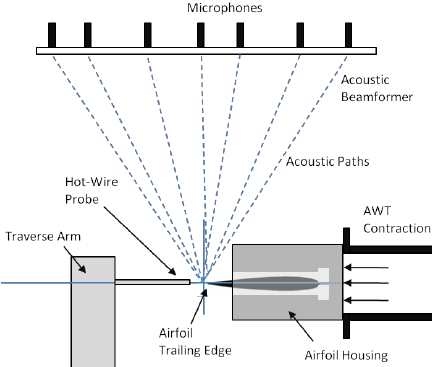
\includegraphics[width=0.5\columnwidth]{schematic-aeroacoustic-beamforming.png}
        \caption{Esquemático de beamforming para um aerofólio. Fonte: \cite{arcondoulis_2010_design}}
    \end{figure}

\end{frame}

% ----------------- NOVO SLIDE --------------------------------


\begin{frame}{Introdução}
    \frametitle{Introdução}
    \framesubtitle{Beamforming e Aprendizado de Máquina}
    \begin{figure}
        \centering
        \begin{tikzpicture}
            [block/.style={draw, text width=2.5cm, align=center}]
            \node (mic) [block] at (0, 0) {Medição do microfone};
            \uncover<-2>{
            \node (beamforming) [block, right=of mic] {Beamforming};
            }
            \visible<3->{
            \node (aprend) [block, below=of beamforming] {Aprendizado de máquina};
            }
            \node (fontes) [block, right=of beamforming] {Fontes de ruído};

            \uncover<-2>{
            \draw [->] (mic) -- (beamforming);
            \draw [->] (beamforming) -- (fontes);
            }
            \visible<3->{
            \draw [->] (mic) |- (aprend);
            \draw [->] (aprend) -| (fontes);
            }

            \visible<2->{
            \node (inputs) [above=0.5cm of mic, green] {Entradas};
            \node [fit=(mic) (inputs), draw, dotted, green, thick] {};
            \node (outputs) [above=0.5cm of fontes, green] {Saídas};
            \node [fit=(fontes) (outputs), draw, dotted, green, thick] {};
            \node (function) [above=0.5cm of beamforming, red] {Função};
            }

            \visible<2>{
            \node [fit=(beamforming) (function), draw, dotted, red] {};
            }
            \visible<3->{
            \node [fit=(function) (aprend), draw, dotted, red] {};
            }
        \end{tikzpicture}
    \end{figure}
\end{frame}

% ----------------- NOVO SLIDE --------------------------------
\section{Objetivos}
\begin{frame}
\frametitle{Objetivos}

Avaliar o uso de
modelos de aprendizado de máquina no
processamento de sinais em
experimentos de aeroacústica;

\begin{enumerate}
    \item Comparar o impacto do tamanho do conjunto de dados de treinamento
        no desempenho do modelo;
    \item Comparar o impacto de diferentes hiperparâmetros no
        desempenho do modelo;
    \item Comparar a acurácia do modelo com a de
        métodos tradicionais de beamforming;
    \item Comparar o tempo computacional com o de
        métodos tradicionais de beamforming;
\end{enumerate}

\end{frame}

% ----------------- NOVO SLIDE --------------------------------
\section{Justificativa}
\begin{frame}{Justificativa}

Os métodos de beamforming são computacionalmente intensos, 
principalmente quando usados com algoritmos de deconvolução
\cite{carranza_2022_beamforming}.
\vspace{5pt}

Sendo uma função que mapeia as leituras dos microfones
às fontes de ruído,
são candidatos a serem substituídos por
aprendizado de máquina.
\vspace{5pt}

Ademais, as redes neurais podem ser projetadas
de modo a diminuir a interferência de ruído,
\cite{ibias2024noise}
aumentando sua acurácia.

\end{frame}

% ----------------- NOVO SLIDE --------------------------------
\section{Referencial Teórico}
\begin{frame}
\frametitle{Referencial Teórico}
\framesubtitle{Aeroacústica linear}

Para calcular a pressão sonora
causada por uma fonte na posição $y$
em um microphone na posição $x$,
serão usadas as seguintes relações \cite{Glegg2023-mi}:

\begin{equation}
    r = |x - y|
\end{equation}

\begin{itemize}
    \item[$x$] posição do microfone
    \item[$y$] posição da fonte
    \item[$r$] distância entre a fonte e o microfone
\end{itemize}

\begin{equation}
    \hat{A} = A \exp(\iu \phi) = A (\cos\phi + \iu \sin\phi)
\end{equation}

\begin{itemize}
    \item[$\hat{A}$] amplitude complexa na fonte
    \item[$A$] amplitude máxima na fonte
    \item[$\phi$] fase da onda
\end{itemize}
\end{frame}

% ----------------- NOVO SLIDE --------------------------------
\begin{frame}
\frametitle{Referencial Teórico}
\framesubtitle{Aeroacústica linear}

\begin{equation}
    \hat{p} = \frac{\hat{A} \exp (\iu k r)}{r}
\end{equation}

\begin{equation}
    k = \frac{\omega}{c}
\end{equation}

\begin{itemize}
    \item[$\hat{p}$] amplitude complexa no ponto $x$
    \item[$\omega$] frequência da onda
    \item[$k$] número de onda (inverso do comprimento de onda)
    \item[$c$] velocidade da onda no meio
\end{itemize}

\end{frame}

% ----------------- NOVO SLIDE --------------------------------
\begin{frame}
\frametitle{Referencial Teórico}
\framesubtitle{Redes Neurais}

\begin{figure}[H]
	\begin{center}
    \begin{tikzpicture}
        \node(i1) [circle, minimum size=22] at (-2, 1) {$i_1$};
        \node(i2) [circle, minimum size=22, below= of i1] {$i_2$};

        \node(12) [draw=black, circle, minimum size=22] at (0, 0) {$+$};
        \node(11) [draw=black, circle, minimum size=22, above=of 12] {$+$};
        \node(13) [draw=black, circle, minimum size=22, below=of 12] {$+$};

        \node(21) [draw=black, circle, minimum size=22, right=of 11] {$+$};
        \node(22) [draw=black, circle, minimum size=22, below=of 21] {$+$};
        \node(23) [draw=black, circle, minimum size=22, below=of 22] {$+$};

        \node(o1) [circle, minimum size=22] at (4, 1) {$o_1$};
        \node(o2) [circle, minimum size=22, below= of o1] {$o_2$};

        \draw[->] (i1) -- (11);
        \draw[->] (i1) -- (12);
        \draw[->] (i1) -- (13);

        \draw[->] (i2) -- (11);
        \draw[->] (i2) -- (12);
        \draw[->] (i2) -- (13);

        \draw[->] (11) -- (21);
        \draw[->] (11) -- (22);
        \draw[->] (11) -- (23);

        \draw[->] (12) -- (21);
        \draw[->] (12) -- (22);
        \draw[->] (12) -- (23);

        \draw[->] (13) -- (21);
        \draw[->] (13) -- (22);
        \draw[->] (13) -- (23);

        \draw[->] (21) -- (o1);
        \draw[->] (21) -- (o2);

        \draw[->] (22) -- (o1);
        \draw[->] (22) -- (o2);

        \draw[->] (23) -- (o1);
        \draw[->] (23) -- (o2);
    \end{tikzpicture} \\
	\caption{\label{fig:ann}Exemplo de rede neural artificial. \fautor}
	\end{center}
\end{figure}

\end{frame}

% ----------------- NOVO SLIDE --------------------------------
\begin{frame}
\frametitle{Referencial Teórico}
\framesubtitle{Redes Neurais}

\begin{figure}[H]
    \centering
    \begin{tikzpicture}
        \node(i2) [circle, minimum size=22] at (-2, 0) {$i_2$};
        \node(i1) [circle, minimum size=22, above= of i2] {$i_1$};
        \node(i3) [circle, minimum size=22, below= of i2] {$i_3$};
        \node(sum) [draw=black, circle, minimum size=22] at (0, 0) {$+$};
        \node(act) [draw=black, minimum size=22] at (2, 0) {$f$};
        \node(out) [circle, minimum size=22] at (4, 0) {$o$};
        \draw[->] (i1) -- (sum) node [midway, above] (TextNode) {$w_1$};
        \draw[->] (i2) -- (sum) node [midway, above] (TextNode) {$w_2$};
        \draw[->] (i3) -- (sum) node [midway, above] (TextNode) {$w_3$};
        \draw[->] (sum) -- (act);
        \draw[->] (act) -- (out);
    \end{tikzpicture} \\
	\caption{Modelo de neurônio. \fautor}
\end{figure}


\end{frame}

% ----------------- NOVO SLIDE --------------------------------
\section{Metodologia}
\begin{frame}
\frametitle{Metodologia}
%\framesubtitle{Usando a suíte abnTeX2}

\begin{figure}[H]
	\begin{center}
	\caption{\label{fig:grid}Esquemático de exemplo de grade de pontos focais e microfones}
    \begin{tikzpicture}[scale=0.8]
        \foreach \x in {1,...,5}
        \foreach \y in {1,...,5}
        %\fill (\x,\y) circle[radius=1pt] node[above right] {$x_{\x,\y}$};
        \fill (\x,\y) circle[radius=1pt] node[above right] {};

        \foreach \x in {1,...,4}
        \draw (\x+0.5,-0.5) circle[radius=2pt] node[above right] {};

        \fill (7, 4) circle[radius=1pt] node[right] {ponto focal};
        \draw (7, 3.5) circle[radius=2pt] node[right] {microfone};
        \draw[draw=black] (6.5,3) rectangle ++(3,1.5);
    \end{tikzpicture} \\
    \fautor
	\end{center}	
\end{figure}


\end{frame}

% ----------------- NOVO SLIDE --------------------------------
\begin{frame}
\frametitle{Metodologia}
\framesubtitle{Hiperparâmetros}

Os hiperparâmetros a serem testados são:
\begin{itemize}
    \item Separação de treino e teste;
    \item Número de camadas escondidas;
    \item Número de neurônios em cada camada escondida;
    \item Número de pares no conjunto de dados;
    \item Porcentagem de pares para treino;
\end{itemize}

\end{frame}


% ----------------- NOVO SLIDE --------------------------------
\section{Resultados preliminares}
\begin{frame}
\frametitle{Resultados preliminares}
%\framesubtitle{Usando a suíte abnTeX2}

Para os testes preliminares foi usada uma grade $6\times6$ pontos focais
e 5 microfones em linha logo abaixo:

\begin{figure}[H]
	\begin{center}
	\caption{Grade usada para os testes preliminares}
    \begin{tikzpicture}[scale=0.8]
        \foreach \x in {1,...,6}
        \foreach \y in {1,...,6}
        %\fill (\x,\y) circle[radius=1pt] node[above right] {$x_{\x,\y}$};
        \fill (-2-1/1.5+\x/1.5,5/6+\y/6) circle[radius=1pt] node[above right] {};

        \foreach \x in {1,...,5}
        \draw (-3+0.2+\x*0.8,0) circle[radius=2pt] node[above right] {};

        \fill (4, 2) circle[radius=1pt] node[right] {ponto focal};
        \draw (4, 1.5) circle[radius=2pt] node[right] {microfone};
        \draw[draw=black] (3.5,1) rectangle ++(3,1.5);
    \end{tikzpicture} \\
    \fautor
	\end{center}	
\end{figure}


\end{frame}

% ----------------- NOVO SLIDE --------------------------------
\begin{frame}
\frametitle{Resultados preliminares}
\framesubtitle{Hiperparâmetros}

Os hiperparâmetros a serem testados são:
\begin{itemize}
    \item Número de camadas escondidas: $ [1] $ 
    \item Número de neurônios em cada camada escondida: $[1, 2, 4, 8, 16, 32, 64, 128, 256, 512, 1024]$;
    \item Número de pares no conjunto de dados: $[100, 180, 325, 585, 1054, 1898, 3420, 6162, 11101, 20000]$
    \item Porcentagem de pares para treino: $[0.25, 0.5, 0.75]$
    \item Taxa de aprendizado: $[1.00e-2, 5.62e-3, 3.16e-3, 1.78e-3, 1.00e-3, 5.00e-4, 3.16e-4, 2.00e-4, 1.41e-4, 1.00e-4, 5.00e-5]$
\end{itemize}

\end{frame}

% ----------------- NOVO SLIDE --------------------------------
\begin{frame}
\frametitle{Resultados preliminares}
\framesubtitle{Treinamento}

\begin{figure}[H]
    \centering
    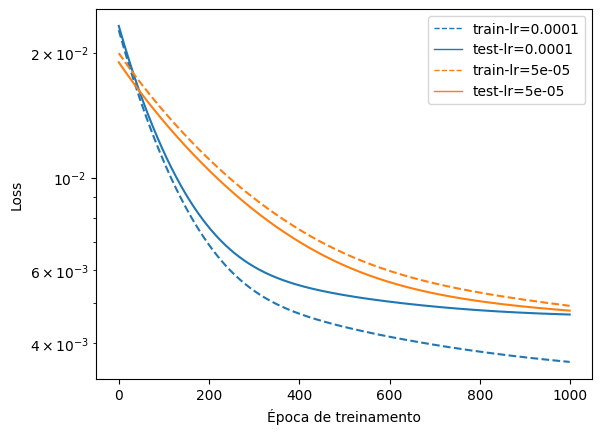
\includegraphics[width=0.5\columnwidth]{loss-ok.png}
    \caption{Treinamento com 32 neurônios e 585 pares de treinamento. \fautor}
\end{figure}

\end{frame}
% ----------------- NOVO SLIDE --------------------------------
\begin{frame}
\frametitle{Resultados preliminares}
\framesubtitle{Treinamento}

\begin{figure}[H]
    \centering
    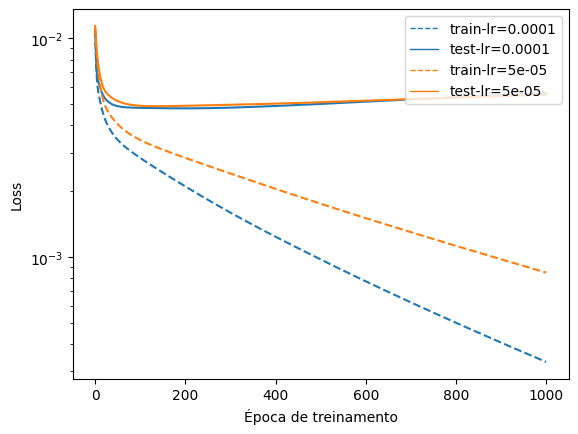
\includegraphics[width=0.5\columnwidth]{loss-overfitting.png}
    \caption{Treinamento com 1024 neurônios e 585 pares de treinamento mostrando overfitting. \fautor}
\end{figure}

\end{frame}

% ----------------- NOVO SLIDE --------------------------------
\begin{frame}
\frametitle{Resultados preliminares}
\framesubtitle{Overfitting}

\begin{figure}[H]
    \centering
    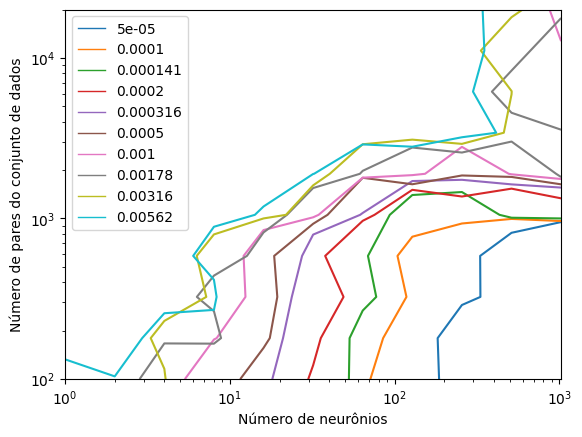
\includegraphics[width=0.6\columnwidth]{overfit.png}
    \caption{Regiões de overfitting. \fautor}
\end{figure}

\end{frame}
% ----------------- NOVO SLIDE --------------------------------
\section{Referências}

% --- O comando \allowframebreaks ---
% Se o conteúdo não se encaixa em um quadro, a opção allowframebreaks instrui 
% beamer para quebrá-lo automaticamente entre dois ou mais quadros,
% mantendo o frametitle do primeiro quadro (dado como argumento) e acrescentando 
% um número romano ou algo parecido na continuação.

\begin{frame}[allowframebreaks]{Referências}
\bibliography{apresentacao}
\end{frame}

% ----------------- FIM DO DOCUMENTO -----------------------------------------
\end{document}
